%! TEX root = ../main.tex
\documentclass[main]{subfiles}

\begin{document}
\chapter{実験3:学習データ数よる予測精度比較}
    \section{目的}
    本研究は,代理モデルによってシミュレーションを予測する.
    しかし,代理モデルは学習データがある程度用意されていないと,予測精度は悪い.
    そのため,はじめはSUMOによるシミュレートによってデータを用意してから代理モデルに切り替える必要がある.
    学習データはより大量にあった方が,代理モデルの精度もより良くなるが,
    学習データを大量に用意するにはより長時間の計算時間が必要になり,代理モデルによって実験の高速化を狙う本研究の目的を達成できなくなる.
    このことから,学習データ数による代理モデルの性能を検証し,代理モデルに切り替えるのはどのタイミングが良いかを決める必要がある.

    \section{実験方法}
    実験2と同様のデータを用いる.このデータは1世代あたり20個の運行スケジュールとその評価値があり,それが100世代存在する.
    1世代目までのデータ,2世代目までのデータ,$\dots$,99世代目までのデータを学習データにし,それぞれの学習データ数の時の予測精度を求める.
    評価指標は決定係数,MAEを用いる.

    \section{結果}
    決定係数を評価指標にした時の予測精度を図\ref{data_1}に示す.
    \begin{figure}
        \begin{minipage}[b]{0.45\linewidth}
          \centering
          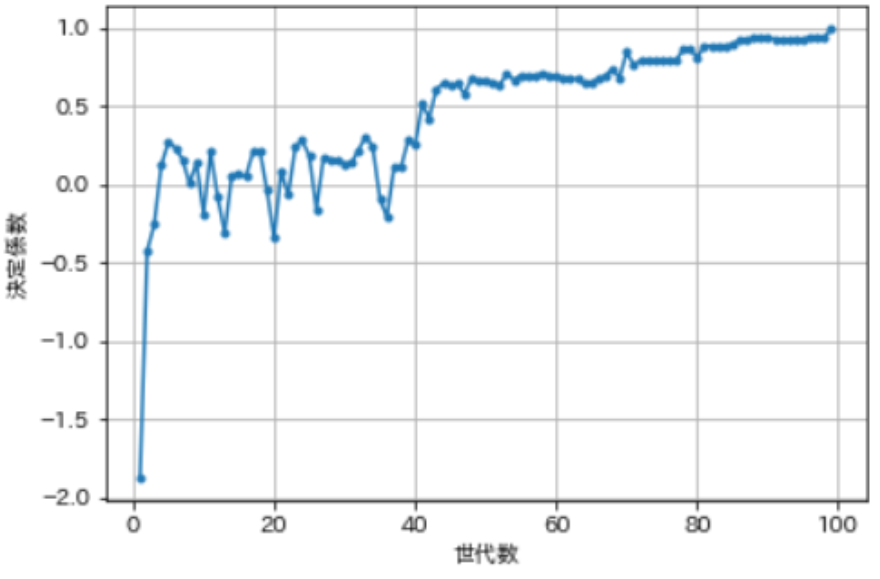
\includegraphics[width=\linewidth]{figures/s_r.png}
          \subcaption{総移動時間}
        \end{minipage}
        \begin{minipage}[b]{0.45\linewidth}
          \centering
          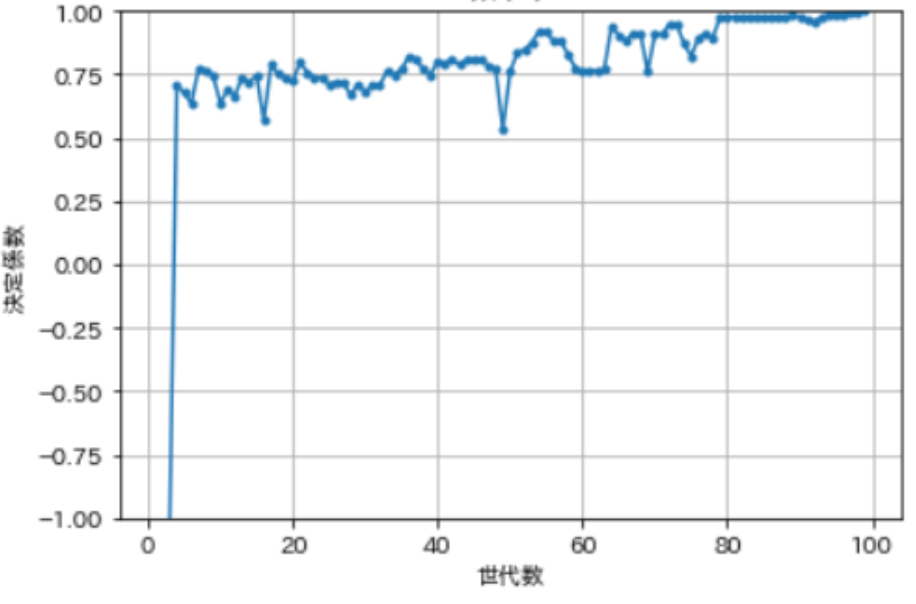
\includegraphics[width=\linewidth]{figures/s_mae.png}
          \subcaption{乗車率}
        \end{minipage}
        \caption{学習データ数による決定係数}
        \label{data_1}
      \end{figure}
      
    MAEを評価指標にした時の予測精度を図\ref{data_2}に示す.
    \begin{figure}
        \begin{minipage}[b]{0.45\linewidth}
          \centering
          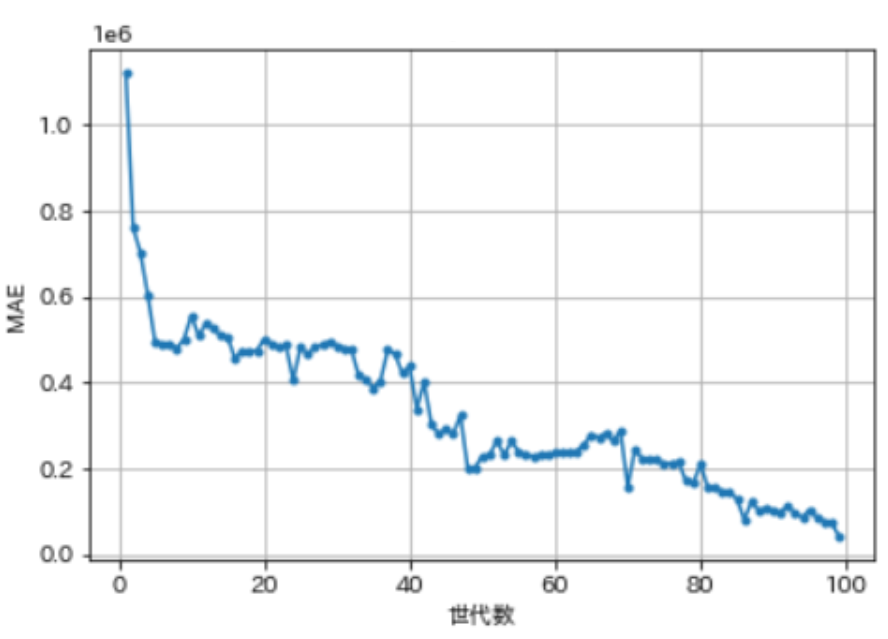
\includegraphics[width=\linewidth]{figures/z_r.png}
          \subcaption{総移動時間}
        \end{minipage}
        \begin{minipage}[b]{0.45\linewidth}
          \centering
          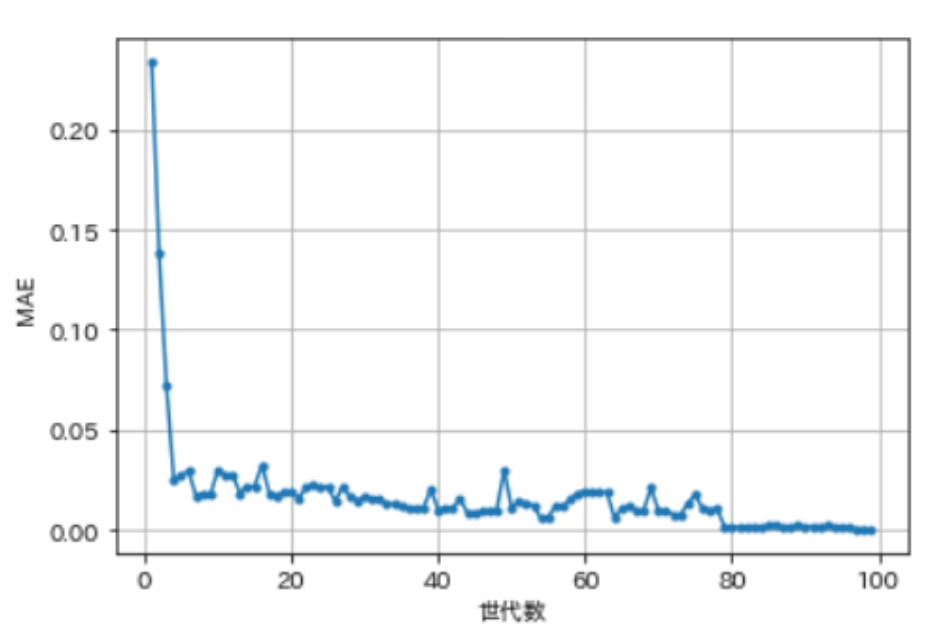
\includegraphics[width=\linewidth]{figures/z_mae.png}
          \subcaption{乗車率}
        \end{minipage}
        \caption{学習データ数によるMAE}
        \label{data_2}
      \end{figure}

\end{document}